\chapter{Огляд стану проблеми та основні поняття}\label{ch:01}

\section{Розвиток та застосування кластеризації}
    Термін ,,кластерний аналіз'', вперше використаний Тріоном у \cite{Tryon:Cluster:1939}, означає набір підходів та алгоритмів, призначених для об'єднання схожих об'єктів у групи. Ця технологія знайшла своє застосування в цілій низці галузей наук та є необхідною частиною більшості сучасних засобів видобування знань.
   
    \begin{figure}
        \centering
        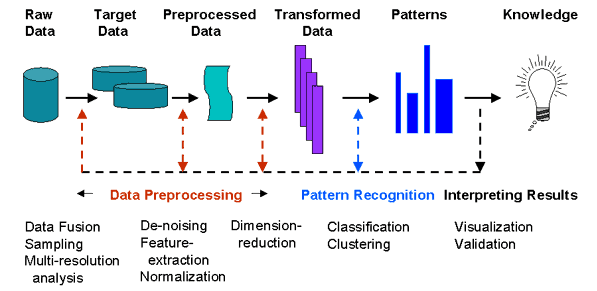
\includegraphics[scale=0.7]{data_mining_steps.png}
        \caption{Етапи видобування даних}\label{fig:data_mining_steps}
    \end{figure}
    
    Рис.~\ref{fig:data_mining_steps} ілюструє етапи процесу видобування знань. Одним із етапів видобування знань є аналіз шаблонів та прихованих закономірностей в базах даних. Саме для пошуку таких закономірностей розроблено алгоритми кластеризації.
 
    В 1959 радянський вчений Терентьєв розробив так званий ,,метод кореляційних плеяд'' \cite{Terentyev}, покликаний здійснювати групування на базі корелюючих ознак об'єктів. Займаючись вивченням кореляцій між різними ознаками озерної жаби, він об'єднав їх в групи за абсолютною величиною коефіцієнту кореляції. Таким чином він отримав дві групи ознак -- ознаки із великим та з малим значенням кореляції. Терентьєв назвав ці групи ,,кореляційними плеядами'' та опублікував декілька методів їх аналізу. Це посприяло розвитку методів кластеризації за допомогою графів.
    
    На початку 50х років також вийшли публікації Р.~Льюїса, Е.~Фікса та Дж.~Ходжеса, присвячені ієрархічним алгоритмам кластеризації. Відчутний поштовх технології кластерного аналізу дали роботи Розенблатта про розпізнаючий пристій ,,перцептрон'' \cite{Rosenblatt}. Ці роботи поклали початок теорії ,,розпізнавання без вчителя''. Поштовхом до розробки методів кластеризації стала публікація \cite{SokalSneath}. В своїй роботі автори Сокел та Сніт виходили з того, що для створення ефективних біологічних класифікацій процедура кластеризації повинна використовувати всеможливі показники, що характеризують досліджувані організми, проводити оцінку ступеня схожості між цими організмами, та забезпечувати розташування схожих організмів в одну групу. При цьому сформовані групи повинні бути досить локальними, тобто схожість організмів всередині групи повинна бути більшою, ніж схожість між організмами, що належать різним групам. Подальший аналіз таких груп допоможе вияснити, чи відповідають вони реальним біологічним класифікаціям. Сокел та Сніт вважали, що виявлення структури розподілу об'єктів у групи допоможе встановити процес утворення цих груп.
    
    В середині сімдесятих з'явилась також низка робіт, присвячених методам аналізу якості здійсненої кластеризації. Індекси Данна \cite{Dunn} та  Девіса-Боулдіна \cite{DavisBouldin} дозволяють чисельно оцінити якість розбиття даних на кластери.

\section{Типові задачі}
    Результатом роботи алгоритмів кластеризації є певне розбиття множини вхідних даних на групи кластери. З кожного із цих кластерів можна виділити типових представників. Це дасть можливість надалі абстрагуватись від великого масиву даних, і при подальшій роботі із таким набором даних працювати не з кожним об’єктом кластера, а лише з таким типовим представником. Такий підхід дозволяє суттєво спростити аналіз даних. Кластеризація часто стає складовою якоїсь більшої задачі, інструментом підготовки даних для її розв'язання. Такі задачі завжди пов'язані із пошуком та виділенням змістовних структур із великих масивів даних. 

    До них можна віднести задачі сегментування та розпізнавання зображень, мовлення, пошуку прихованих закономірностей в даних. На практиці такі задачі виникають при розв'язуванні проблем, що виникають в медицині, соціології, економіці та низці інших сфер діяльності людини. 
    У медицині, наприклад, техніка сегментування зображення дозволяє виділяти на томограмах окремі області і на підставі їх форми та забарвлення приймати ставити діагноз. В біології використовуються техніки кластеризації для виявлення взаємопов'язаних груп генів та їх впливу на живі організми. Кластеризація також успішно застосовується у маркетингових дослідженнях для виявлення зв'язків між різними групами споживачів та потенційних покупців, цільових аудиторій, та для оптимального позиціонування нової продукції. 
    В соціологічних дослідженнях використовується кластеризація даних, отриманих з різних джерел, для спрощення їх подальшого аналізу. 

    У своїй праці \cite{Zagorujko} Загоруйко описує одну із таких задач. Новосибірські вчені вивчали причини переселення людей з сіл в міста. Були вислані експедиції в навколишні села, жителям яких задавали приблизно сто анкетних питань, що стосувались віку, сімейного становища, освіти та ін. Після завершення опитування дослідники постали перед необхідністю аналізувати більш ніж сім тисяч анкет, що містили понад сто питань кожна. 
    Ці дані було введено в програму таксономії, котра повернула сім великих таксонів, середні характеристики яких дозволили дати зібраним даним змістовну інтерпретацію. Наприклад, виділився кластер, що містив переважно жінок середнього віку, котрі мали дорослих дітей в місті. Очевидно, представниці цього таксону, названого дослідниками ,,бабусі'', їхали в місто доглядати за своїми внуками. Решту таксонів опрацьовано аналогічно.
    
    Перед процедурою кластеризації часто дані буває необхідно підготувати. В практиці нормою є випадки, коли для деяких об'єктів бракує частини атрибутів -- в такому разі перед кластеризацією необхідно здійснити передбачення цих атрибутів, користуючись наявною інформацією. Також значення атрибутів об'єктів необхідно нормувати.

\section{Основні поняття та означення}
    Дамо математичне означення кластеризації. Нехай $D$ -- множина об'єктів. 
    \begin{definition}
        \emph{Кластеризацією} $C = \{C \mid C \subseteq D\}$ називається таке розбиття $D$ на множини, 
        для якого виконується $\cup_{C_i \in C} = D$ і $\forall C_i, C_j \in C : C_i \cap C_{j \neq i} = \emptyset$. 
        Множини $C_i$ називаються кластерами.
    \end{definition}
    Як вже згадувалось раніше, задача кластеризації полягає в знаходженні такого розбиття $C$, щоб схожі між собою об'єкти належали до одного кластера, а не схожі - до різних. Необхідно визначити спосіб обчислення схожості об'єктів.
    Для цього на просторі об'єктів вводиться певна метрика, геометричний зміст якої -- відстань між об'єктами. Вона використовується як величина, обернена до міри схожості між об'єктами. На даний момент розроблено і широко застосовується наступний набір метрик:
    \begin{itemize}
        \item {евклідова відстань} 
            \begin{equation}
                \rho(x, x') = \sqrt{ \sum_{i=1}^n (x_i - x_i')^2}
            \end{equation}
        \item {квадрат евклідової відстані} 
            \begin{equation}
                \rho(x, x') = \sum_{i=1}^n (x_i - x_i')
            \end{equation}
            (використовується для надання більшої ваги об'єктам, розташованим далеко один від одного)
        \item {манхеттенська відстань} 
            \begin{equation}
                \rho(x, x') = \sum_{i=1}^n \mid x_i - x_i' \mid
            \end{equation}
        \item {відстань Чебишева}
            \begin{equation}
                \rho(x, x') = max(\mid x_i - x_i' \mid )
            \end{equation}            
            ця метрика дозволяє розрізнити об'єкти, якщо вони відрізняються лише одною координатою
    \end{itemize}
    
    
    
\section{Алгоритми кластеризації}
    На даний момент значного розвитку набула ціла низка різноманітних алгоритмів кластеризації. Їх можна розділити на групи за різними ознаками:
    \begin{itemize}
        \item спосіб групування (роздільне, ієрархічне)
        \item визначеність 
        \item чутливість до форми кластерів 
    \end{itemize}
    
    Роздільні алгоритми будують одне розбиття вибірки на кластери. На відміну від роздільних, агломеративні будують цілу систему взаємовкладених кластерів. На виході алгоритму отримується дерево кластерів, коренем якого служить кластер, що містить усі об'єкти вибірки, а листками є найменші кластери, кожен з яких містить по одному об’єкту. В такому разі дослідник має можливість обрати такий переріз дерева кластерів, що найкраще відповідатиме його потребам.
    
    Визначені алгоритми однозначно ставлять у відповідність кожному об'єкту один кластер. Невизначені не дають такої чіткої інформації. Замість ідентифікатора кластера вони повертають імовірність, із якою об'єкт належить до кожного із кластерів.
    
    На сьогоднішній день широко використовуються наступні алгоритми кластеризації:
    \begin{itemize}
        \item k-means \cite{Steinhaus, MacQueen}
        \item UPGMA \cite{SokalMichener}
        \item DBSCAN \cite{DBSCAN}
        \item FOREL \cite{Zagorujko}
        \item c-means
        \item карти Кохонена \cite{Rosenblatt}
    \end{itemize}
    
\section{Висновки до розділу 1}
    Нині набула поширення низка практичних задач, розв’язання яких вимагає виявлення прихованих закономірностей у наборі даних. Задачі такого типу виникають у медицині, соціології, економіці та низці інших галузей людської діяльності. Кластеризація набула великого значення як засіб розв’язання таких задач. У зв’язку із розвитком інформаційних технологій спостерігається значне зростання об’ємів даних, що піддаються збору та обробці. Така тенденція вимагає створення ефективних алгоритмів кластеризації, здатних обробляти масиви даних великого об’єму.
    
    У першому розділі наведено відомості про розвиток алгоритмів кластеризації до сьогоднішнього дня. Також у цьому розділі подано означення основних понять, пов’язаних із задачами кластеризації, та формальне означення самого поняття кластеризації. У 1.3 описано популярні алгоритми кластеризації та їх розбиття на групи за кількома критеріями.
    
    Для здійснення кластеризації необхідно визначити метрику простору, міру відстані між об’єктами вибірки. В розділі наведено декілька основних та найпопулярніших метрик, що нині використовуються для кластеризації.
